\documentclass{article}
\usepackage[utf8]{inputenc}
\usepackage[T1]{fontenc}
\usepackage{lmodern} % Arrête définitivement la boucle de messages METAFONT
\usepackage{amsmath}
\usepackage{amssymb}
\usepackage{amsthm}
\usepackage{amsfonts}
\usepackage{graphicx}
\usepackage{amstext}
\usepackage{amsopn}

% --- CONFIGURATION DES CHEMINS D'ACCÈS AUX IMAGES ---
\graphicspath{
    {images/TDA/}
    {images/phase_final_repulsive/}
    {images/phase_final_adhesive/}
}

\title{Internship Progress}
\author{aurelien astesiano}
\date{April 2026}

\begin{document}

\maketitle

\section{Code}

\subsection{Parameters}

\begin{itemize}
\item $u_0$ (1.0) : Self-propulsion speed
\item $r_R$ (0.075) : Agent-agent repulsion radius, below which agents repel each other.
\item $r_A$ (0.1) : Maximum distance at which an agent aligns with other agents.
\item $\nu$ (2.0) : Alignment intensity (in front of the target vector).
\item $\tau$ (0.15) : Distance below which an agent starts to feel the presence of an obstacle and repel it.
\item $C_{\phi}$ (5.0) : Agent-obstacle repulsion intensity
\item $d_s$ (0.02) : Noise on orientation
\item $\eta$ (1.0) : Viscosity felt by the obstacles
\item $d_o$ (0.0) : Noise on obstacles set to 0 by default
\item $\kappa$ \textbf{variable} (10, 100 or 1000) : Obstacle spring stiffness.
\item $\mu$ \textbf{variable} Agent-agent repulsion intensity.
\item $\zeta$ \textbf{variable} Viscosity on agents.
\item $M$ Number of agents set to 3000 by default
\item $N$ Number of obstacles set to 3000 by default
\item $L$ Length of an edge set to 1 by default
\item $dt$ Discretization in the Euler scheme, set to 0.005 by default but we will implement an adaptive time step (see below)
\end{itemize}

\subsection{Grid}

We consider the maximum interaction radius of an agent with its surroundings, which is the maximum between $r_a$, $r_r$, and $\tau$. We divide the total size by this parameter to get the number of cells.\\
We create an array that counts the number of elements per grid cell and an array that gives the indices of the elements in each cell of the grid.\\
We fill it with a loop over the agents; for each, we take the integer part of their position divided by the cell size. We then get the cell in which the agent is located, and we add 1 to the corresponding counter for that cell. We do the same for the obstacles.

\subsection{Forces}

We start with the agent-obstacle potential:
$$
\phi(x) = \frac{3C_\phi}{2\pi\tau} \left(1 - \frac{|x|}{\tau}\right)_+^2
$$
which gives the force gradient applied each time:
$$
F_\phi(x) = -\nabla \phi(x) = \frac{3C_\phi}{\pi\tau^2} \left(1 - \frac{|x|}{\tau}\right) \frac{\vec{x}}{|x|}
$$
Thus, in the code, we keep the prefactor constant in memory.
\\
Same thing for the agent-agent repulsion:
$$
\psi(x) = \frac{6\mu}{\pi r_R^2} \left(1 - \frac{|x|}{r_R}\right)_+^2
$$
Which gives the inter-agent force:
$$
F_\psi(x) = -\nabla \psi(x) = \frac{12\mu}{\pi r_R^3} \left(1 - \frac{|x|}{r_R}\right) \frac{\vec{x}}{|x|}
$$
and we keep the prefactor in memory.

\subsection{Hooke's Spring Stability}
Since the force can be very strong (stiff spring), we use an exponential Euler scheme, for which the proof of the formula used in the code is given here:\\
Let $U(t) = X_i(t) - Y_i$ be the distance from the obstacle to its anchor point and $a = \frac{\kappa}{\eta}$. Assuming the external force $F_{ext}$ is constant over the interval $[t, t+\Delta t]$ (which is indeed the case in our discretization), the differential equation for the obstacles is written as:
$$\frac{dU}{dt} = -a U(t) + F_{ext}$$
Multiplication by the integrating factor $e^{at}$:
$$e^{at} \frac{dU}{dt} + a e^{at} U(t) = e^{at} F_{ext}$$
$$\frac{d}{dt} \left( U(t) e^{at} \right) = e^{at} F_{ext}$$
Integration over the interval $[t, t+\Delta t]$:
$$U(t+\Delta t) e^{a(t+\Delta t)} - U(t) e^{at} = F_{ext} \int_{t}^{t+\Delta t} e^{as} ds$$
$$U(t+\Delta t) e^{a(t+\Delta t)} - U(t) e^{at} = F_{ext} \frac{e^{a(t+\Delta t)} - e^{at}}{a}$$
Multiplication by $e^{-a(t+\Delta t)}$ to isolate $U(t+\Delta t)$ :$$U(t+\Delta t) = U(t) e^{-a\Delta t} + F_{ext} \frac{1 - e^{-a\Delta t}}{a}$$
Deduction of the exact displacement of the obstacle over the time step, $\Delta X_i = U(t+\Delta t) - U(t)$:$$\Delta X_i = U(t)(e^{-a\Delta t} - 1) + F_{ext} \frac{1 - e^{-a\Delta t}}{a}$$

The factors in front of U(t) and $F_{ext}$ are calculated at initialization in the code; then, to obtain the displacement of an obstacle during $\Delta t$, we apply the formula above. The external forces being the obstacle-agent interactions.

\subsection{Angle Variation}
In the code, we use the angle value on the trigonometric circle rather than the vector. Using the fact that:
$$J_k = \sum_{|Z_k - Z_j| \le r_A} \alpha_j = \begin{pmatrix} \sum \cos\theta_j \\ \sum \sin\theta_j \end{pmatrix}$$
and
$$\tan(\bar{\theta}_k) = \frac{Y}{X} = \frac{\sum \sin\theta_j}{\sum \cos\theta_j}$$
To find the mean theta, we use the appropriate Python function arctan2, which avoids non-bijection and division by 0 issues; it is defined as follows:
$$\text{arctan2}(Y, X) = \begin{cases} \arctan(\frac{Y}{X}) & \text{if } X > 0 \\ \arctan(\frac{Y}{X}) + \pi & \text{if } X < 0 \text{ and } Y \ge 0 \\ \arctan(\frac{Y}{X}) - \pi & \text{if } X < 0 \text{ and } Y < 0 \\ \frac{\pi}{2} & \text{if } X = 0 \text{ and } Y > 0 \\ -\frac{\pi}{2} & \text{if } X = 0 \text{ and } Y < 0 \end{cases}$$

Once we have this angle, we apply the orthogonal projection in the following way:
$$\nu \bar{\alpha}_k \cdot \alpha_k^\perp = \nu \begin{pmatrix} \cos\bar{\theta}_k \\ \sin\bar{\theta}_k \end{pmatrix} \cdot \begin{pmatrix} -\sin\theta_k \\ \cos\theta_k \end{pmatrix}$$

$$\nu \bar{\alpha}_k \cdot \alpha_k^\perp = \nu (\sin\bar{\theta}_k \cos\theta_k - \cos\bar{\theta}_k \sin\theta_k) = \nu \sin(\bar{\theta}_k - \theta_k)$$

The calculation above is literally translated into the code.

\subsection{Adaptive dt}
To be able to support an adhesive force that will create high concentrations, it is necessary to add an adaptive time step.
For this, we calculate the maximum speed of all agents during this iteration (this is the last step of the loop, all forces having been calculated beforehand) and we arbitrarily set:
$$dt_{ideal} = \frac{0.3 * r_{min}}{v_{max}}$$
Where $r_{min}$ is the minimum interaction radius so that with this dt we cannot "jump through" an interaction.\\
In this case, we choose a fraction of time to advance that is lower than $dt_{ideal}$.\\
Since the simulation sometimes explodes in complexity, we add dividing the time step by 10 as an absolute minimum limit.\\
With this compromise, the simulations do not take too much time and have a coherent output.

\subsection{Tip}
For agent-agent interactions (repulsion and alignment), since they are symmetric, we only look at the top and right cells and process the double interaction directly, which halves the computation time for these forces.\\
The while loop and the time as a parameter of the function allow, during display, to simply advance by the precisely desired time, and the function will reach it, making it possible to record at regular intervals.

\section{Adhesive Case}
To switch to the adhesive case, we simply add a minus in front of the agent-obstacle repulsion force. We can later discuss the relevance of this new force, as it stability issues when the distance between an agent and an obstacle approaches 0.

\subsection{Micro Simulation Results}
We will try to reproduce the results from the article but in the adhesive case with the same parameters. In the phase diagrams, we vary the agent-agent repulsion ($\mu$), which increases from left to right, and the viscosity on the agents ($\zeta$), which increases from bottom to top.

\begin{figure}[hbp!]
    \centering
    \begin{minipage}{0.48\textwidth}
        \centering
        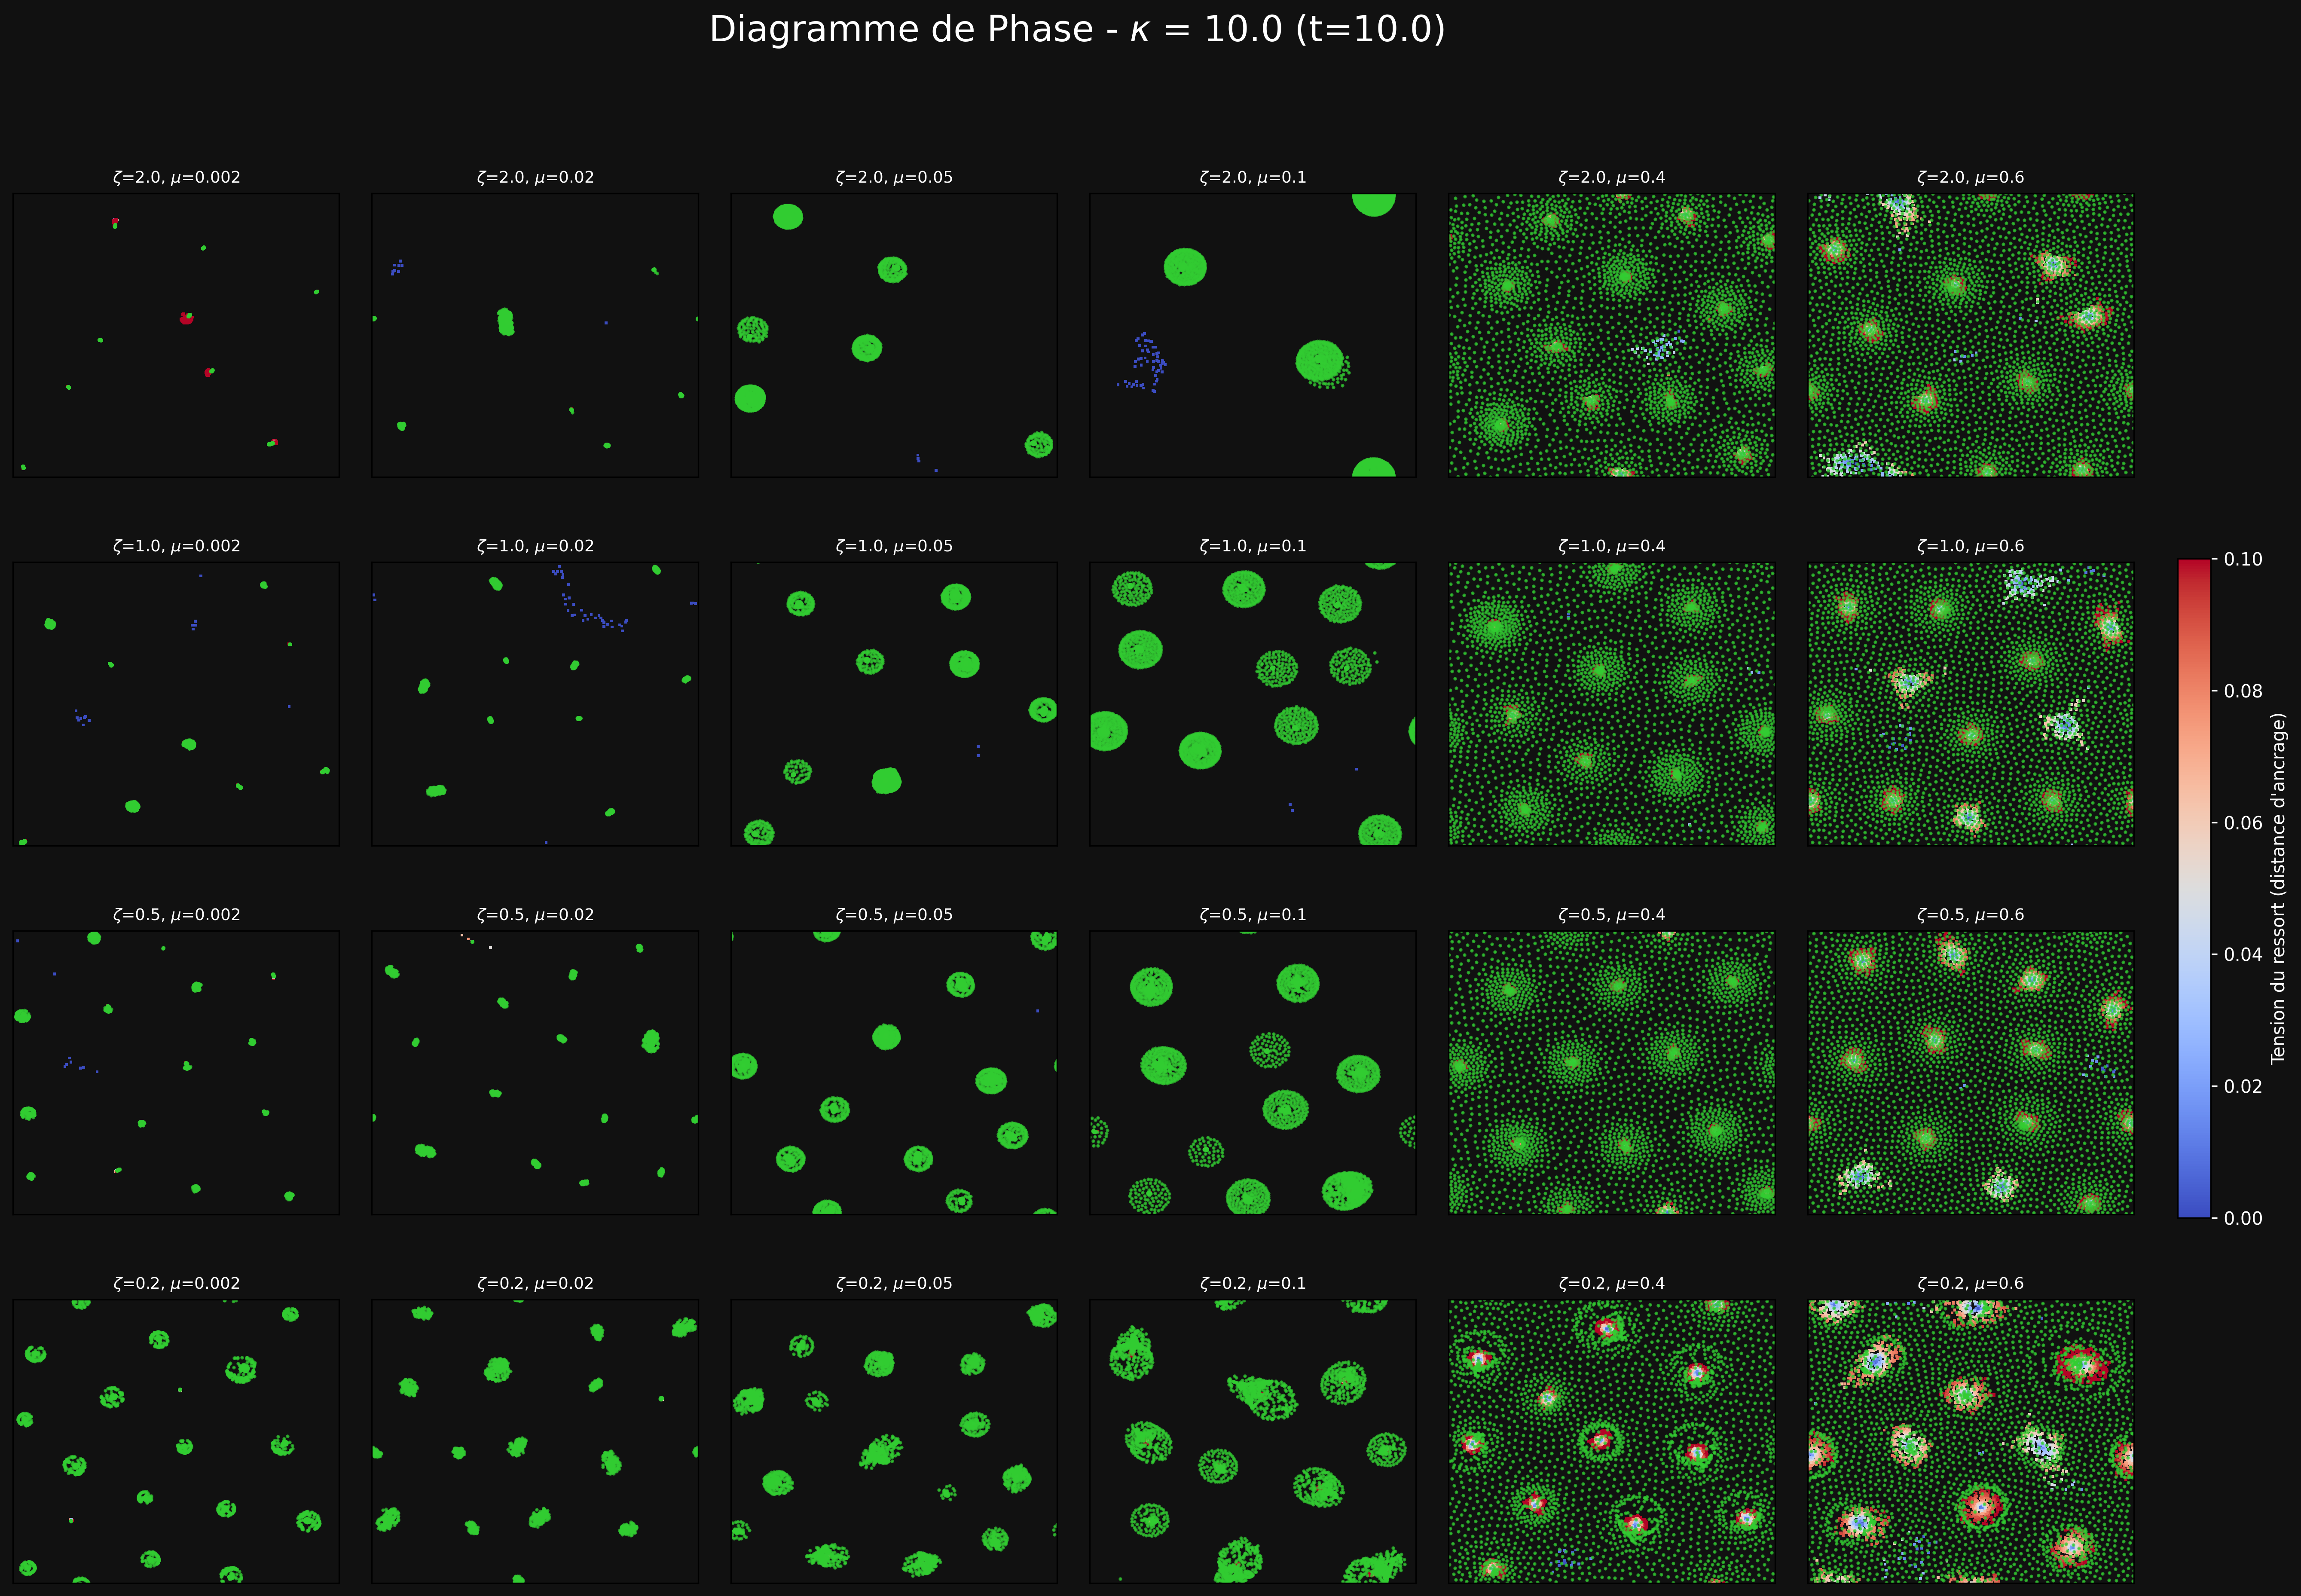
\includegraphics[width=\linewidth]{phase_diagram_kappa_10.png}
        \caption{Simulation (Adhesive model) - $\kappa = 10$}
        \label{fig:sim_k10}
    \end{minipage}\hfill
    \begin{minipage}{0.48\textwidth}
        \centering
        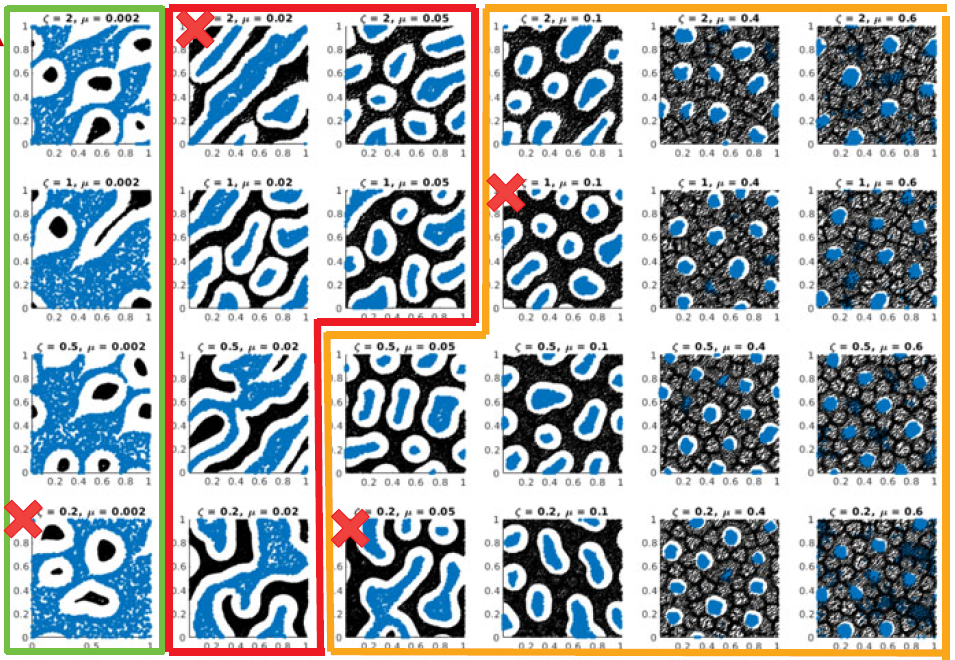
\includegraphics[width=\linewidth]{kappa_10_article.png}
        \caption{Article - $\kappa = 10$, $\zeta$ = [2.0, 1.0, 0.5, 0.2], $\mu$ = [0.002, 0.02, 0.05, 0.1, 0.4, 0.6]}
        \label{fig:art_k10}
    \end{minipage}
\end{figure}

\textit{Analysis ($\kappa=10$):} Here we can clearly see the split between the first 4 columns, from which clusters can emerge, and the next two, where this is no longer possible. Only the cluster size varies, and only the case zeta = 2 and mu = 0.05 shows 2 moving clusters. A parallel with honeycombs can be seen in the last two columns, even though the obstacles are already concentrated in the previous ones.

\begin{figure}[hbp!]
    \centering
    \begin{minipage}{0.48\textwidth}
        \centering
        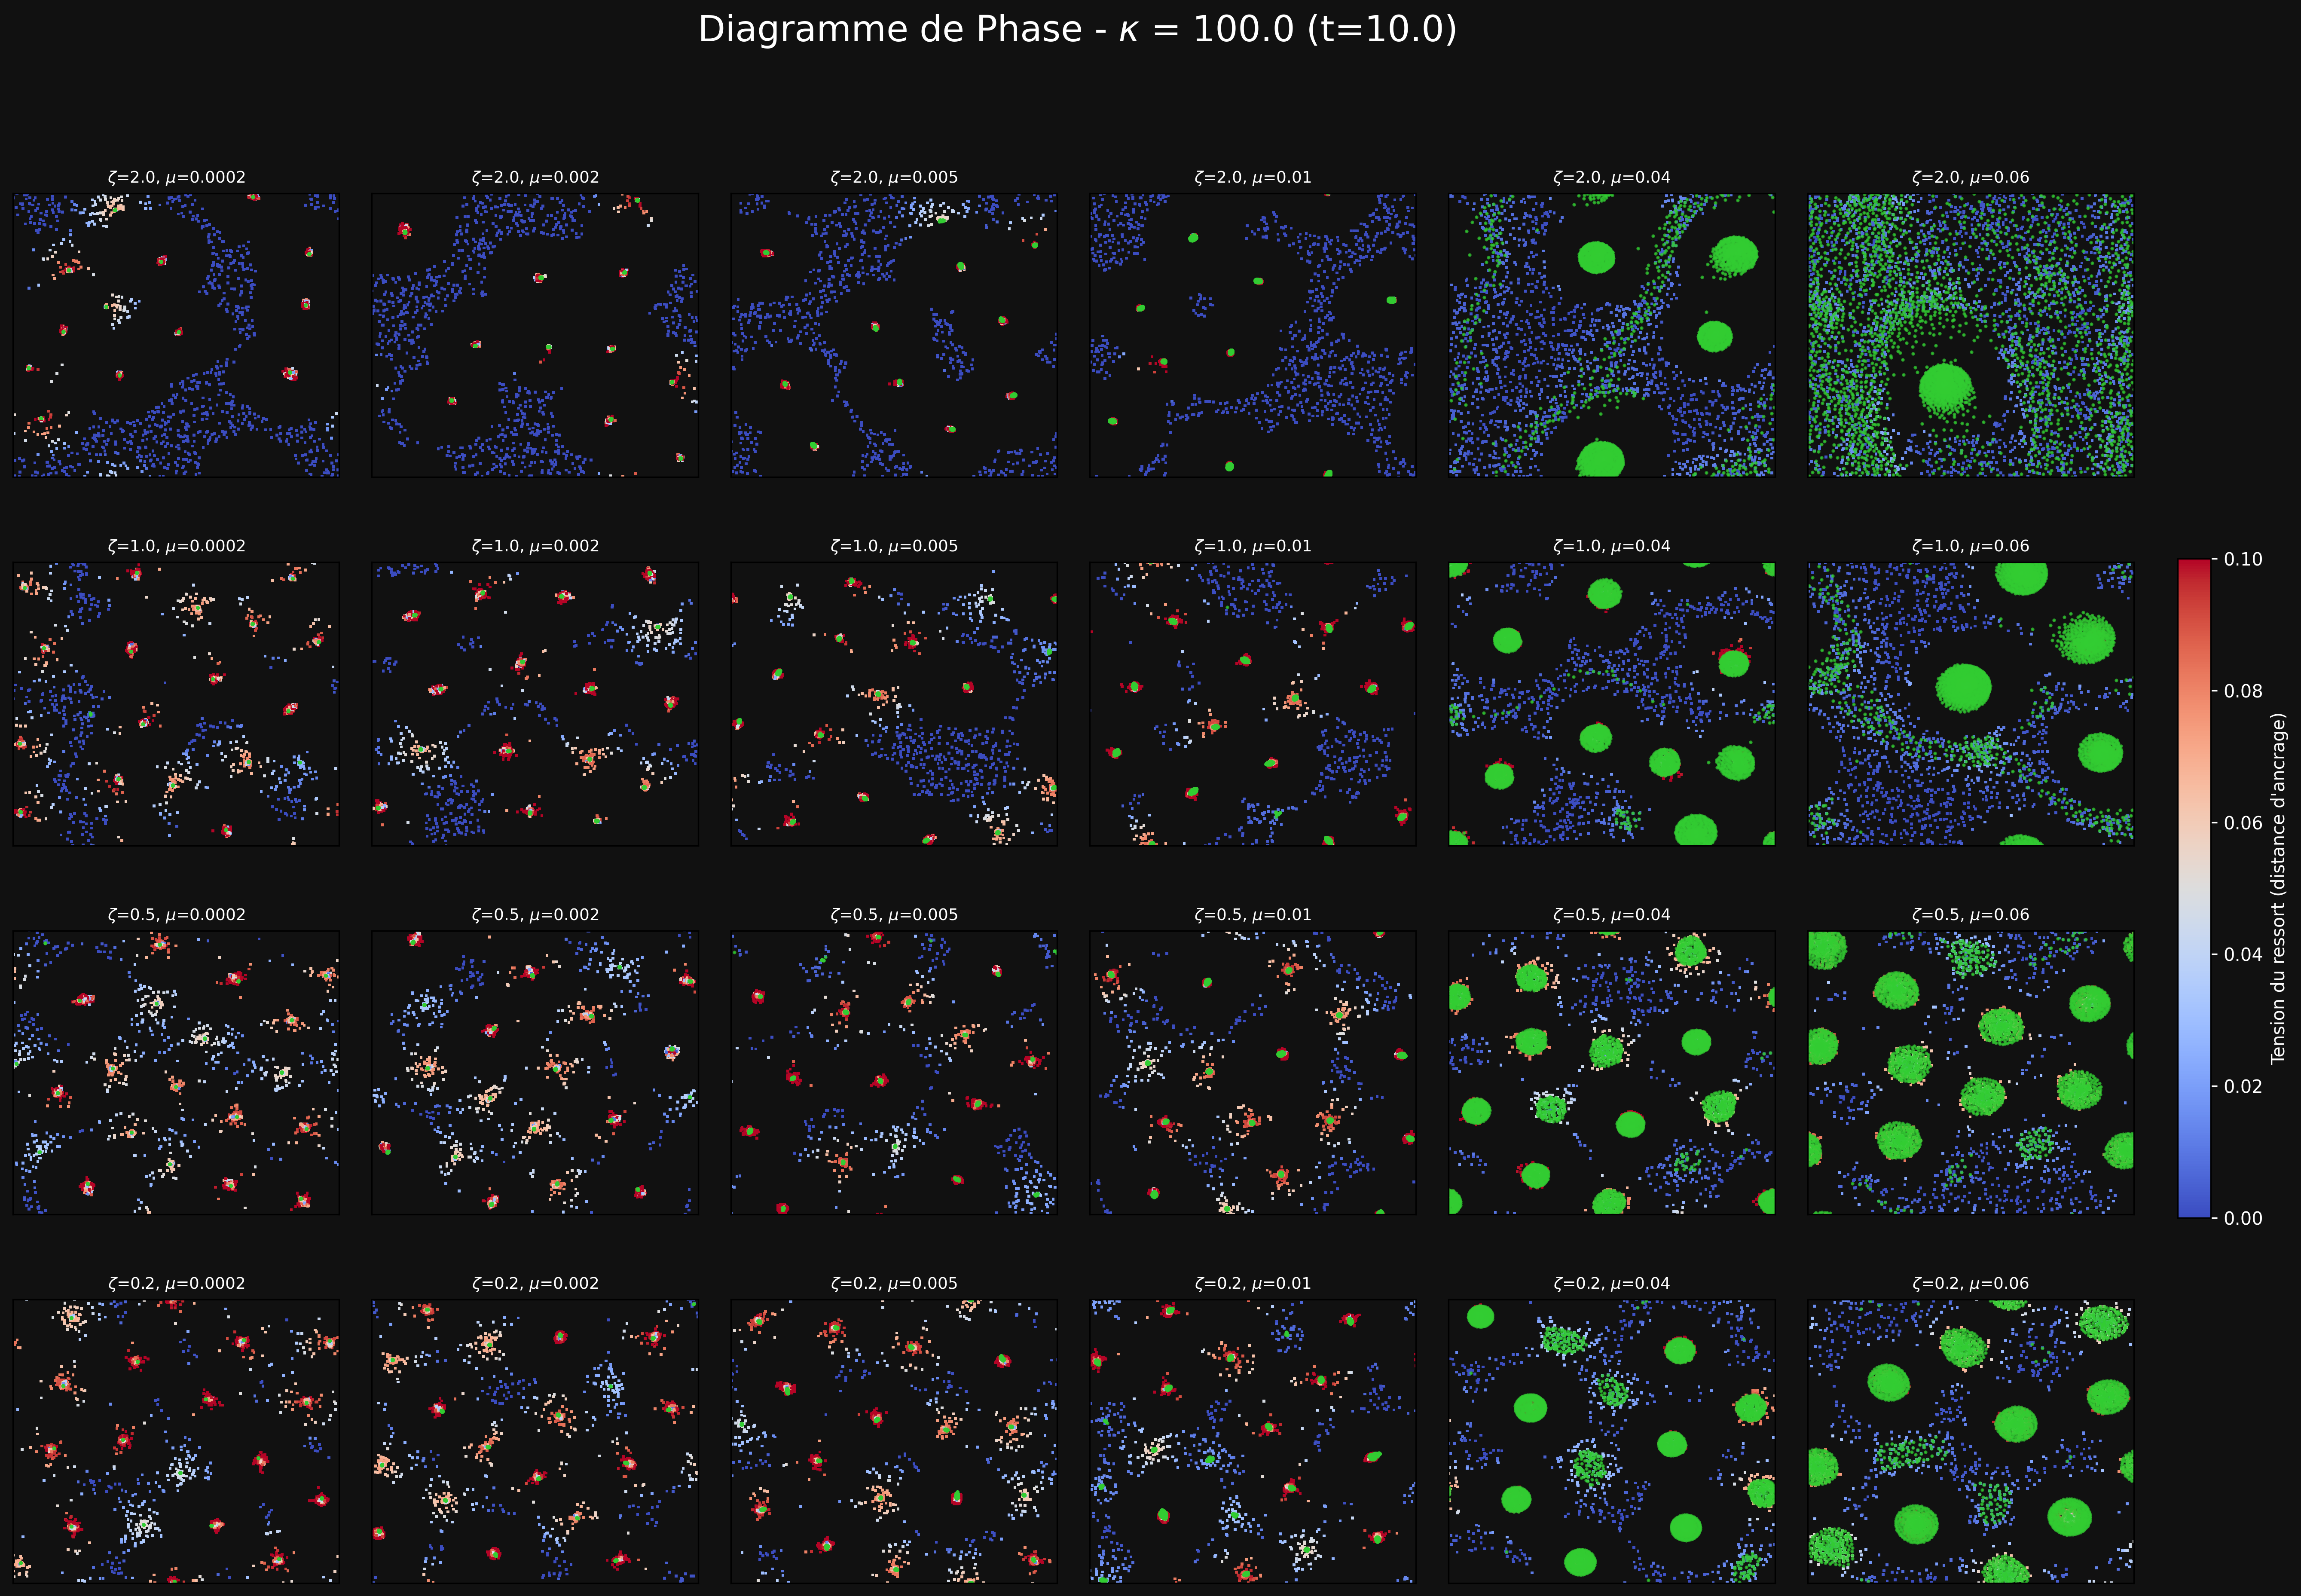
\includegraphics[width=\linewidth]{phase_diagram_kappa_100.png}
        \caption{$\kappa = 100$, cells are green and obstacles range from blue to red through white depending on the distance to their anchor point}
        \label{fig:sim_k100}
    \end{minipage}\hfill
    \begin{minipage}{0.48\textwidth}
        \centering
        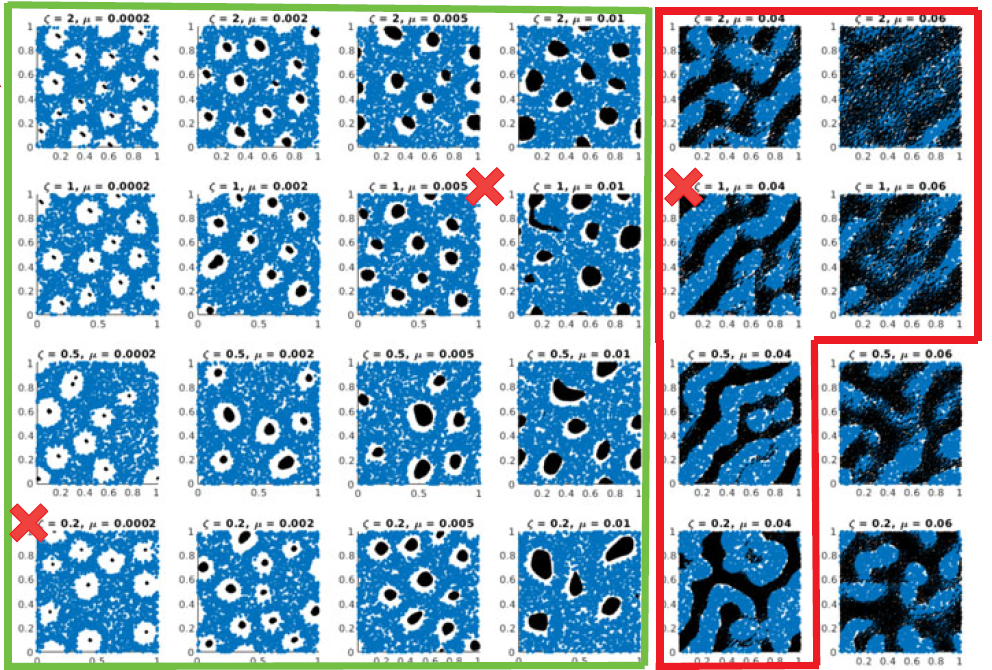
\includegraphics[width=\linewidth]{kappa_100_article.png}
        \caption{Article - $\kappa = 100$, $\zeta$ = [2.0, 1.0, 0.5, 0.2], $\mu$ = [0.0002, 0.002, 0.005, 0.01, 0.04, 0.06]}
        \label{fig:art_k100}
    \end{minipage}
\end{figure}

\textit{Analysis ($\kappa=100$):} Here the cells gather tightly around fixed but unstable concentrated points, so some can move until they find an equilibrium point depending on the distribution of surrounding obstacles. In the last two columns, there are still cells that have a track movement following the obstacles; however, clusters still emerge (strong predominance of clusters in the bottom right, coexistence in the top right). In the top right, they are no longer clusters that suck in particles forever, but rather particles enter and leave them via self-propulsion.

\begin{figure}[hbp!]
    \centering
    \begin{minipage}{0.48\textwidth}
        \centering
        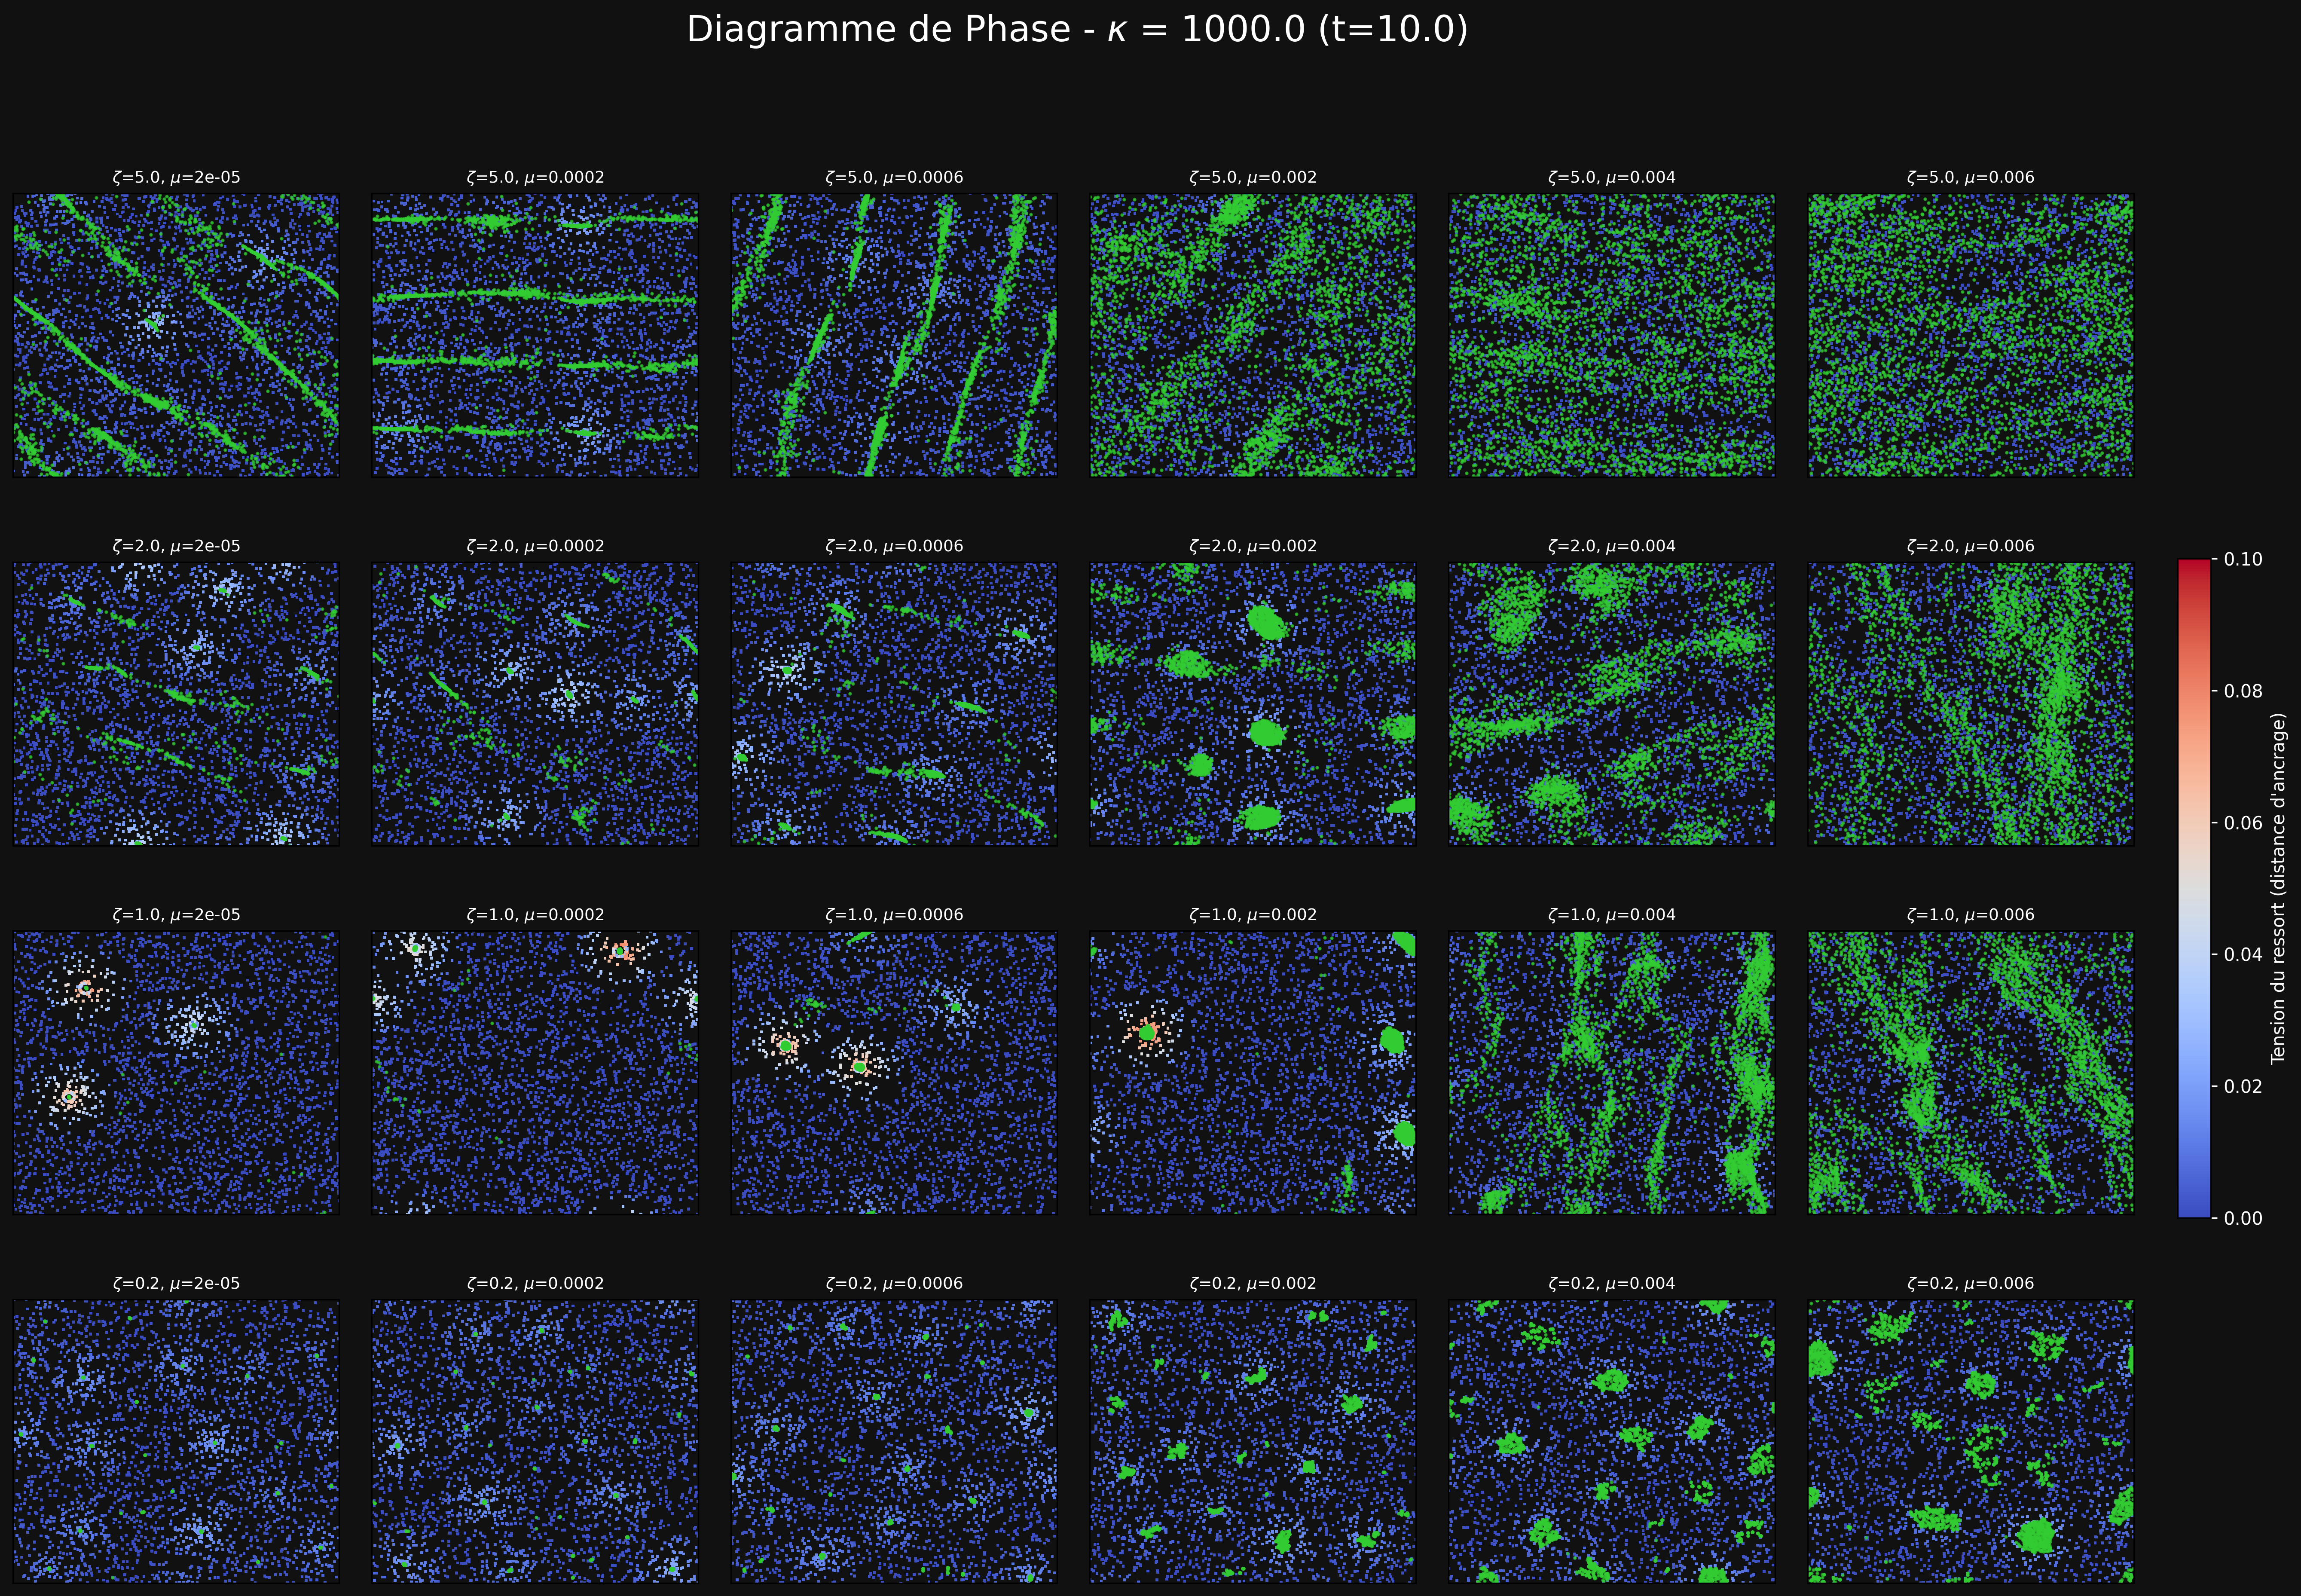
\includegraphics[width=\linewidth]{phase_diagram_kappa_1000.png}
        \caption{$\kappa = 1000$}
        \label{fig:sim_k1000}
    \end{minipage}\hfill
    \begin{minipage}{0.48\textwidth}
        \centering
         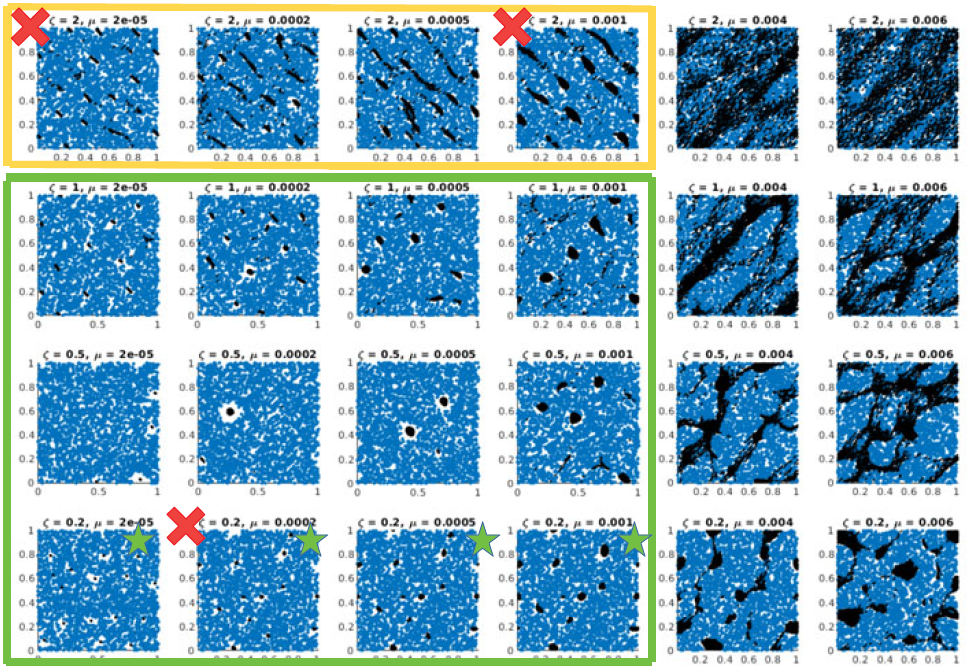
\includegraphics[width=\linewidth]{kappa_1000_article.png}
        \caption{Article - $\kappa = 1000$, $\zeta$ = [5.0, 2.0, 1.0, 0.2], $\mu$ = [2e-5, 2e-4, 6e-4, 2e-3, 4e-3, 6e-3]}
        \label{fig:art_k1000}
        \end{minipage}
\end{figure}

\textit{Analysis ($\kappa=1000$):} In this case, the observed behavior is extremely similar. On the first row, the clusters are fixed as in the article; however, this occurs across the entire row, but in the last two, some cells are fixed and others are moving. Above, the clusters are moving, so the results are really very similar.


\subsection{Future Developments}
\begin{itemize}
\item Numerical instability: For now, with the lower limit on the time step, we maintain a local instability. To resolve it, we will try to remove the lower bound on the time step and add a condition that when the distance between the particle and the obstacle is extremely small (less than $10e^{-12}$), the force is zero. I will run tests again and recreate a phase diagram to see if we obtain differences and if the simulations are coherent.
\item Once the instabilities are resolved, we can move towards a more advanced comparison between adhesion and repulsion. The analysis would focus on when differences arise between adhesion and repulsion. To do this, I will first understand and reuse the geometrically invariant quantifiers used in the article to analyze the results. Once this is done, it will be necessary to determine the regions to test and the questions we want to answer.
\item This ties into the point above, but there is also an avenue to explore regarding the initial distribution of obstacles; we can imagine distributions in bands, spheres, or other shapes and observe the differences.
\end{itemize}

\section{Comparison adhesive/repulsive}
\subsection{Choice of the distance}
We will focus here on the different type of distances that can be used to observe patterns differences (or not) between to images. Then we will compare them over a data set.
\subsubsection{Wasserstein 1D}
As done in the article we can take two discrete distributions, project them on a grid with same size (we will talk about optimal grid size later) and compare the wasserstein distance of there signatures. Making it totally space invariante only depending on the repartition of the cells.

\subsubsection{Fourier}
to have a distance considering geometric we can think of using fourier transform of our density, the intuition is that it will be very efficient to see difference between bandes and clusters for exemple. We put our two discrete models on a thin grid (also discussion on the choice of the grid) and we take the spectrum of this density. To compare two densities we can take L2 difference of their spectrum.

\subsubsection{Topological data analysis}
The objective is to map a point cloud to a mathematical vector characterizing its global shape. Based on an article that directly applied this framework to active matter, we explain the general principle.

We start with a point cloud consisting of coordinates $X = \{r_1, r_2, \dots, r_K\}$ in a 2D space.

Mathematically, we define building blocks called \textit{simplices}:
\begin{itemize}
    \item A $0$-simplex is a point.
    \item A $1$-simplex is a line segment connecting two points.
    \item A $2$-simplex is a solid triangle (composed of 3 points).
\end{itemize}
\begin{figure}
    \centering
    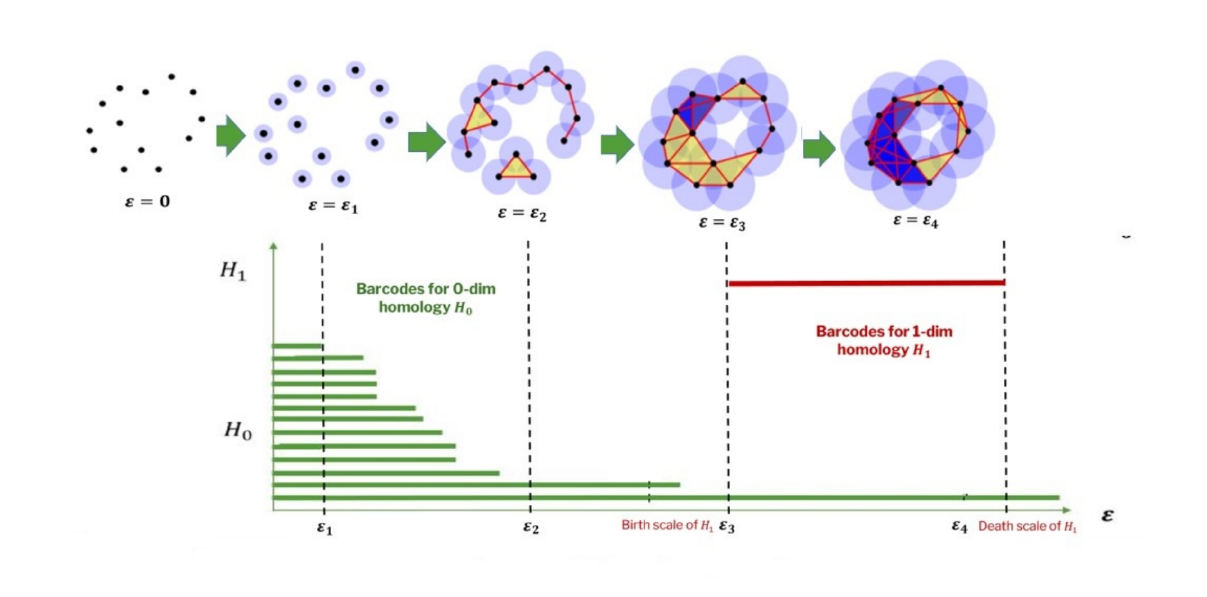
\includegraphics[width=1\linewidth]{filtration.png}
    \caption{filtration}
    \label{fig:filtration_tda}
\end{figure}
\paragraph{The Connection Rule (Filtration)}
We imagine a ball of diameter $\epsilon$ around each point. We gradually increase this scale parameter $\epsilon$ starting from $0$:
\begin{itemize}
    \item If two balls overlap (meaning the distance between the two points is less than the defined threshold), we create an edge (a $1$-simplex).
    \item If three edges form a closed triangle, we fill it to create a face (a $2$-simplex).
\end{itemize}

We then analyze two homology groups:
\begin{itemize}
    \item \textbf{The $H_0$ group:} It represents the connected components (clusters or islands).
    \item \textbf{The $H_1$ group:} It represents 1D holes (loops). A hole is "born" when edges form a closed cycle without a solid face inside, and it "dies" when $\epsilon$ is large enough for faces (triangles) to completely fill this empty space.
\end{itemize}

\paragraph{Persistence (The Barcode)}
For each topological feature (an $H_0$ island or an $H_1$ hole), the algorithm records two fundamental values:
\begin{itemize}
    \item Its \textbf{birth ($b$)} at a given scale $\epsilon$.
    \item Its \textbf{death ($d$)} when the feature disappears or merges with a larger one.
    \item Its \textbf{persistence $P = d - b$}, which measures the "lifespan" or robustness of this topological feature.
\end{itemize}

\paragraph{Persistence Landscapes}
Next, we must transform these "barcodes" into exploitable data. To do so, "tent functions" are used. Considering continuous values of the scale parameter $\epsilon$, these functions are defined for each interval $(b,d)$ as:

\begin{equation}
    h_{(b,d)}(\epsilon) = \max\left\{0, \frac{P}{2} - |\epsilon - \frac{b+d}{2}|\right\}
\end{equation}

\begin{figure}
    \centering
    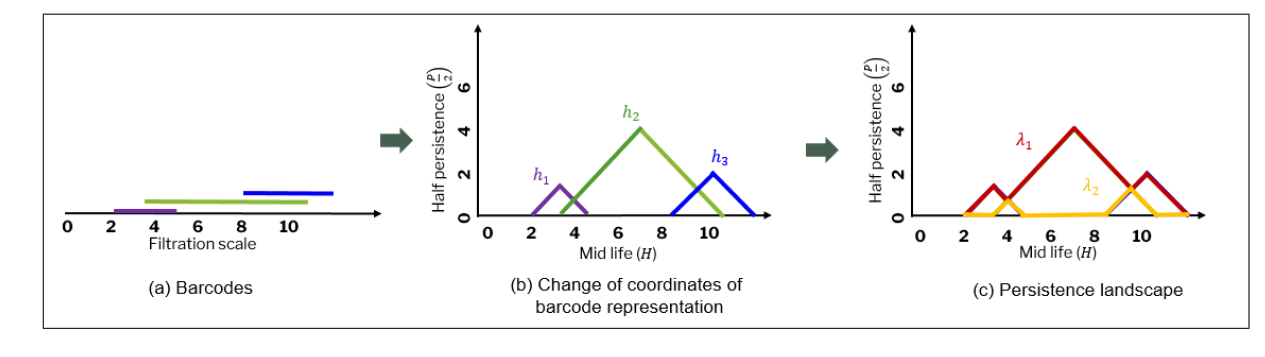
\includegraphics[width=1\linewidth]{Persistence_landscapes.png}
    \caption{barcode and landscapes}
    \label{fig:landscapes_tda}
\end{figure}

From these functions, we define the $m$-th upper envelope, which corresponds to the $m$-th largest value at a given $\epsilon$ (see figure). This yields a persistence landscape composed of $\{\lambda_1, \lambda_2, \dots, \lambda_M\}$. The integer $M$ is deliberately chosen to be relatively small to filter out topological noise, keeping only the features that persist long enough (i.e., tall tent functions).

We can then compute the persistence landscape contour (or average landscape):
\begin{equation}
    L(\epsilon) := \frac{1}{M'} \sum_{m=1}^{M'} \lambda_m(\epsilon)
\end{equation}

Using theoretical results established in the literature, $L(\epsilon)$ is proven to be a continuous function on a bounded interval $[0, \epsilon_{max}]$, belonging to a normed vector space (the $L^p$ space). This provides the mathematical justification to treat these landscapes as standard Euclidean vectors.

\paragraph{Vectorization and Comparison}
In practice, this function is not evaluated continuously. We define a regular grid of resolution $K$ over the studied interval, such that $\epsilon_k = k \cdot \Delta\epsilon$ for $k \in \{1, \dots, K\}$. The continuous function $L(\epsilon)$ is sampled to become a vector in $\mathbb{R}^K$:
\begin{equation}
    \vec{V} = [L(\epsilon_1), L(\epsilon_2), \dots, L(\epsilon_K)]
\end{equation}

At this stage, the reference article performs a series of statistical tests tailored to their specific objectives. However, for our specific goal of comparing two distinct simulations (e.g., simulation A and B), we can simply compute the Euclidean difference:
\begin{equation}
    \text{Distance} = ||\vec{V}_A - \vec{V}_B||_2
\end{equation}
This topological distance can then be plotted on a graph as a function of each physical parameter we wish to investigate.

\paragraph{Adaptation : Periodic Cubical Homology on Density Fields}

We change the filtration because VR seems to not work, this method is too sensitive to microscopic fluctuations and isolated particules. To robustly capture the macroscopic structures we will use the \textbf{Cubical Complex} method.
\\
Unlike the Vietoris-Rips this method has to be done for a density on a grid. To track the topological features of the density, we use a superlevel set filtration.\\

Let $\rho(x,y)$ be the local density of active agents. For a given density threshold $\epsilon$, the superlevel set is the region of the domain where the density is greater than or equal to the threshold:
\begin{equation}
    \mathcal{X}_\epsilon = \{ (x,y) \in \text{Grid} \mid \rho(x,y) \geq \epsilon \}
\end{equation}
Instead of growing balls around points, the filtration parameter $\epsilon$ starts at the global maximum density and progressively decreases to zero :
\begin{itemize}
    \item \textbf{Birth:} When the decreasing threshold $\epsilon$ hits a local density peak, an isolated cluster of active particles emerges, creating a new connected component in the $H_0$ homology group.
    \item \textbf{Death:} As $\epsilon$ continues to decrease, these initially isolated high-density islands expand. When two clusters intersect on the grid, they merge. The younger component "dies" and gets absorbed by the older component.
\end{itemize}
Computationally we will take $-\rho$ and apply functions from gudhi library were everything is implemented.

\subparagraph{Vectorization via Betti Curves}
Instead of Persistence Landscapes, we vectorize the barcodes using Betti Curves. The Betti curve $\beta_0(\epsilon)$ is a step function defined simply as the rank (or Betti number) of the homology group at a given threshold $\epsilon$ so :
\begin{equation}
    \beta_0(\epsilon) = \text{rank}(H_0(X_\epsilon))
\end{equation}
This curve directly counts the number of independent clusters existing at the density threshold $\epsilon$. The following is the same as before.

\subsection{comparison on test}
\subsubsection{typical atterns}
First, I generate 6 typical patterns to compare how those 3 distances are differenciating them. I made an heatmap which is on the github testing all the pairs and writing the distance associated. We have uniform state, large bandes, thin bandes, trails, big clusters, little clusters.\\
We are making a little analysis of the result for each distance.
\begin{itemize}
    \item \textbf{TDA} : Lower distance is between uniform state and large bandes, second is between little clusters and large clusters which is positive because we want to have them in the same type of pattern. However it is making a significant distance between large bandes and thin bandes.
    \item \textbf{Fourier} : Two smallest distance are between large bandes and uniform state then between small clusters and large clusters. It seems to work the same as TDA except that it captures less the difference between large bandes and trails but this is not an issue because cells oientation is an easy way to differenciate those two.
    \item \textbf{Wasserstein} : For wasserstein distance, in average the ratio between the smallest distance and the higher distance is two times more than the two other measures. Wasserstein quite not see the difference between trails and thin bandes and between uniform states and large bandes. It is penalising more than the others the difference between small clusters and large clusters.
\end{itemize}

\textbf{Conclusion} : Finally, all distance are little between large bandes and uniform state which is not an issue beacause we can see on the image that the bands clearly exists but are not very distinct. Each one have it's own specifity, for the next test, huge distance between small clusters and huge clusters will be an issue but as showed the heatmap on other patterns wasserstein could be more efficient.

\subsubsection{Emergence of difference between adhesion and repulsion}
We try to find a parameter region where at the beginning patterns are the same and when change a set of parameter patterns are changing. To comparate patterns difference we will use the three distances explained before.\\
After unsuccessfully changing only the stiffness or trying to vary the parameter epsilon over the scaling assumption of macro-regime, a test that worked pretty well was to keep to ratio constant :
    \begin{itemize}
        \item $\kappa \mu$ : This ratio called $b_p$ in the article played the key role of pattern emergence. We had to keep it less than 1 to see pattern emergence.
        \item $\frac{\mu}{\zeta}$ : This ratio is the term in front of agent-agent force, we can think that keeping it constant could help keeping the same patterns for differents parameters but there is no rigorous proof...
    \end{itemize}
We start at $\kappa$ = 1000 on a regime where agents are making bandes for one and clusters for another, then we are reducing the $\kappa$ = 10 . To describe quickly the results :
\begin{itemize}
    \item for bandes for long time we have stable bandes for both for long time, then for $\kappa \leq 100$ we can see instabilities emerging creating clusters than captures agents and obstacles around them so the final result is extremly different between adhesive and repulsive and this what we expect to see for the 3 distances (low distance for $200 \leq \kappa \leq 1000$ and huge for $\kappa \leq 100$).
    \item for clusters at the beggining it is very similar and then for repulsive case it is slightly becoming trails (pinned clusters then moving clusters larger and larger and then connected trails) so we want to observe a progressive augmentation for $\kappa$ from 1000 to 10.
\end{itemize}
We plot a comparison between the three distances here
\end{document}